\documentclass[11pt, a4paper]{article}
\usepackage[margin=2cm]{geometry}
\usepackage{enumitem}
\usepackage{booktabs}
\usepackage{hyperref}
\usepackage{graphicx}
\usepackage{tabularx}
\usepackage{longtable}
\usepackage{array}
\usepackage{titling}
\setlength{\parskip}{2pt}
\setlist{nosep, leftmargin=*}

\hypersetup{
    colorlinks=true,
    linkcolor=blue,
    urlcolor=blue
}

\title{\textbf{Assignment 2: Plan, Design, Deploy}\\[0.5em]
\large Software Project --- Spring 2026}
\author{}
\date{}

\begin{document}
\maketitle
\thispagestyle{empty}

\begin{center}
\begin{tabular}{ll}
\toprule
\textbf{Project} & PoetryForYou --- Telegram Poetry Learning Bot \\
\textbf{Customer} & Nursultan Askarbekuly \\
\textbf{Team Member} & Egor Zhukov \\
\textbf{Role} & Solo Developer (Full-stack, DevOps, QA, Research) \\
\bottomrule
\end{tabular}
\end{center}

\subsection*{What I Did This Week}
\begin{enumerate}
    \item Derived user stories from the Week~1 interview and prioritized them with MoSCoW.
    \item Created a Use Case diagram and ER diagram based on the initial data model.
    \item Designed the REST API (4 endpoints) and documented it with example requests/responses.
    \item Set up the GitHub repo and created issues as the product backlog (16 PBIs).
    \item Deployed MVP~v0 to an Aeza VPS --- the bot responds to \texttt{/start} and runs the onboarding flow.
    \item Wrote this report and prepared the Postman collection.
\end{enumerate}

% ============================================================
% USE CASE DIAGRAM
% ============================================================

\section{Use Case Diagram}

\begin{center}
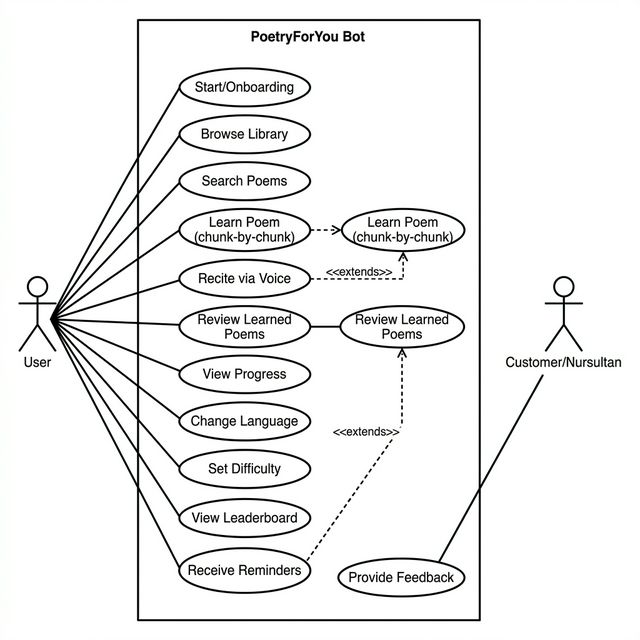
\includegraphics[width=0.85\textwidth]{use_case_diagram.png}
\end{center}

The diagram shows 12 use cases for two actors. The \textbf{User} interacts with the bot for onboarding, browsing the library, learning poems chunk-by-chunk, reciting via voice, reviewing, viewing progress, changing language/difficulty, and viewing the leaderboard. The \textbf{Customer} provides feedback on the product. ``Recite via Voice'' extends ``Learn Poem'' (voice is an optional way to practice). ``Receive Reminders'' extends ``Review Learned Poems'' (reminders trigger reviews).

% ============================================================
% USER STORIES
% ============================================================

\section{User Stories (Product Backlog)}

User stories are derived from the customer interview (Week~1). Prioritized with MoSCoW, estimated in Story Points (SP).

\begin{center}
\footnotesize
\begin{longtable}{|p{0.38\textwidth}|c|c|c|}
\hline
\textbf{User Story} & \textbf{Priority} & \textbf{SP} & \textbf{Issue} \\
\hline
\endhead
As a user, I want to start with \texttt{/start} so the bot greets me and asks my language. & Must & 2 & \#1 \\
\hline
As a user, I want to set my difficulty level so poems match my ability. & Must & 2 & \#2 \\
\hline
As a user, I want to browse a poem library so I can pick what to learn. & Must & 5 & \#3 \\
\hline
As a user, I want to learn a poem chunk-by-chunk so I don't get overwhelmed. & Must & 8 & \#4 \\
\hline
As a user, I want to test my memory via text so the bot checks my answer. & Must & 5 & \#5 \\
\hline
As a user, I want to recite via voice message so I practice speaking. & Must & 8 & \#6 \\
\hline
As a user, I want a similarity score after reciting so I know my accuracy. & Must & 3 & \#7 \\
\hline
As a user, I want the bot to search poems online so I'm not limited to built-in ones. & Should & 5 & \#8 \\
\hline
As a user, I want spaced repetition reminders so I don't forget poems. & Should & 5 & \#9 \\
\hline
As a user, I want to view my learning progress so I stay motivated. & Should & 3 & \#10 \\
\hline
As a user, I want to switch between RU and EN interface. & Should & 3 & \#11 \\
\hline
As a user, I want to see a leaderboard to compare with others. & Could & 3 & \#12 \\
\hline
As a user, I want the bot to recommend poems based on my preferences. & Could & 5 & \#13 \\
\hline
As a user, I want to set my display name for the leaderboard. & Could & 2 & \#14 \\
\hline
As a user, I want to pause and resume learning across sessions. & Must & 3 & \#15 \\
\hline
As a user, I want \texttt{/help} to list all available commands. & Must & 1 & \#16 \\
\hline
\end{longtable}
\end{center}

\textbf{Product Backlog:} \href{https://github.com/d13-l1t3/PoetryForYou/issues}{GitHub Issues (link)} --- 16 issues, labeled by priority.

% ============================================================
% DESIGN
% ============================================================

\section{Design}

\subsection*{Data Model (ER Diagram)}

\begin{center}
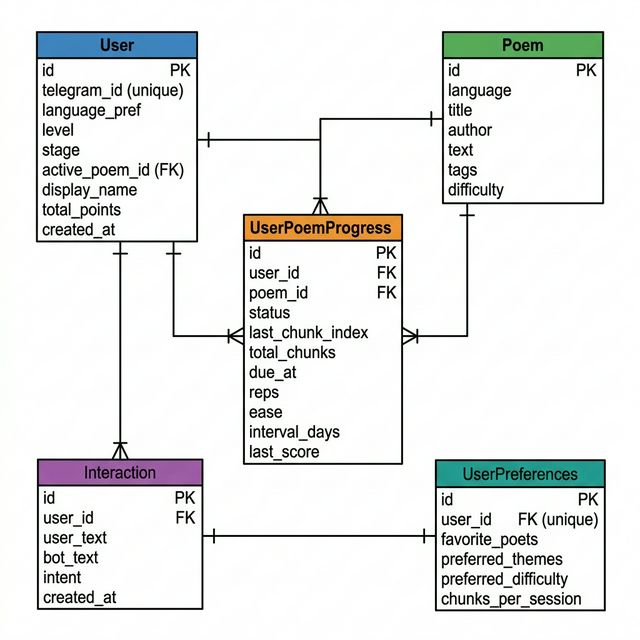
\includegraphics[width=0.9\textwidth]{er_diagram.png}
\end{center}

Five entities: \textbf{User} stores Telegram ID, language, level, and gamification points. \textbf{Poem} holds the text, author, tags, and difficulty. \textbf{UserPoemProgress} tracks chunk-based learning state and spaced repetition parameters (SM-2 algorithm). \textbf{Interaction} logs every message exchange. \textbf{UserPreferences} stores favorite poets, themes, and learning pace. Relationships: User 1:N UserPoemProgress, Poem 1:N UserPoemProgress, User 1:N Interaction, User 1:1 UserPreferences.

\subsection*{UI Prototype}

Figma prototype: \href{https://FIGMA_LINK_HERE}{Figma prototype (link)}.

Five screens: (1)~Onboarding --- language selection, (2)~Onboarding --- difficulty selection, (3)~Main menu with reply buttons (\texttt{/learn}, \texttt{/library}, \texttt{/review}, \texttt{/progress}), (4)~Chunk-based learning --- showing poem lines and asking to type from memory, (5)~Voice recitation result --- similarity score and feedback.

\subsection*{API Design}

Four REST endpoints. Postman collection with examples: \href{https://POSTMAN_LINK_HERE}{Postman mock (link)}.

\begin{center}
\footnotesize
\begin{tabularx}{\textwidth}{l|l|X}
\toprule
\textbf{Method} & \textbf{Endpoint} & \textbf{Description} \\
\midrule
GET & \texttt{/health} & Health check. Returns \texttt{\{"ok": true\}}. \\
POST & \texttt{/message} & Main text endpoint. Body: \texttt{\{telegram\_id, text\}}. Returns \texttt{\{reply, intent, stage\}}. \\
POST & \texttt{/voice} & Voice upload (multipart/form-data). Fields: \texttt{telegram\_id} + audio file. Whisper STT, then processes like \texttt{/message}. Max 10~MB. \\
POST & \texttt{/cleanup} & Internal: cleanup expired sessions, persist progress. \\
\bottomrule
\end{tabularx}
\end{center}

% ============================================================
% DEPLOYMENT
% ============================================================

\section{MVP v0 Deployment}

\textbf{Live bot:} \href{https://t.me/PoetryforYou_bot}{@PoetryforYou\_bot}

\textbf{Repository:} \href{https://github.com/d13-l1t3/PoetryForYou}{github.com/d13-l1t3/PoetryForYou}

\textbf{Stack:} Python (FastAPI + python-telegram-bot) + PostgreSQL + Docker Compose. Deployed on Aeza VPS (Ubuntu 24.04, 1 vCPU, 2 GB RAM).

\textbf{How to run:} \texttt{git clone} $\rightarrow$ \texttt{cp .env.example .env} $\rightarrow$ fill tokens $\rightarrow$ \texttt{docker compose up --build -d}.

\textbf{Current state:} Bot handles \texttt{/start} onboarding (language + difficulty), poem browsing, chunk-based learning, voice recitation with Whisper, progress tracking, and bilingual UI (RU/EN).

% ============================================================
% ACTIVITY TRACKING
% ============================================================

\section{Activity Tracking}

\begin{center}
\begin{tabular}{|l|l|r|}
\hline
\textbf{Day} & \textbf{Activity} & \textbf{Hours} \\
\hline
Mon & Reviewed A1 feedback, derived user stories from interview & 2 \\
\hline
Tue & Created Use Case diagram, wrote ER diagram from data model & 2 \\
\hline
Wed & Designed API, created Postman collection with examples & 1.5 \\
\hline
Thu & Set up GitHub Issues backlog (16 issues with labels) & 1.5 \\
\hline
Fri & Deployed MVP~v0 to VPS, tested end-to-end & 3 \\
\hline
Sat & Wrote the report, prepared diagrams and deliverables & 2 \\
\hline
\multicolumn{2}{|r|}{\textbf{Total}} & \textbf{12} \\
\hline
\end{tabular}
\end{center}

% ============================================================
% CUSTOMER FEEDBACK
% ============================================================

\section{Customer Feedback}

Based on the customer interview from Week~1, the following requirements guide this week's design decisions:

\begin{itemize}
    \item The \textbf{core flow} (browse $\rightarrow$ learn $\rightarrow$ recite $\rightarrow$ score) is the highest priority. Gamification comes later.
    \item The bot must feel like a \textbf{conversation}, not a web app. Reply buttons and natural dialogue are key.
    \item \textbf{Voice recitation checking} with edge-case handling (mumbling, skipped lines) is the main engineering challenge.
    \item \textbf{Two languages} (RU + EN) are required, with Russian as the primary focus.
    \item The customer expects \textbf{2--3 intermediate demos} before the final exam on March~25.
    \item MVP~v0 is deployed and ready for the first demo feedback.
\end{itemize}

% ============================================================
% AI USAGE
% ============================================================

\section{AI Usage}

I used ChatGPT to help format the user stories into a table and to generate the ER diagram layout. The Postman collection was built from the running API. Use Case diagram, prioritization (MoSCoW), and all design decisions are my own work based on the customer interview.

\end{document}
